% =============================================================================
% ANEXOS
% =============================================================================

% ---------------------------------------------------------------------------
% NOTA: Los anexos contienen material de referencia y evidencia complementaria.
% Las secciones principales del sistema se mencionan en el cuerpo de la tesis
% con referencia a "ver Anexo X" cuando el detalle excede el espacio del cuerpo.
% ---------------------------------------------------------------------------

%%─────────────────────────────────────────────
\chapter{Capturas de pantalla del sistema}
\label{anexo:capturas}
%%─────────────────────────────────────────────

Este anexo complementa la sección~\ref{sec:prototipo} del Capítulo~5
documentando las vistas de los roles Secretario y Miembro de la Comisión
Curricular, el flujo de usuario con múltiples roles, y las pantallas
secundarias de funcionalidades avanzadas del sistema.

%%────────────────────────────────────────────────────────────────────────────
\section{Vista del Secretario}
\label{anexo:vista_secretario}
%%────────────────────────────────────────────────────────────────────────────

El Secretario opera principalmente sobre la gestión administrativa de
propuestas: puede consultar el estado de todas las propuestas, gestionar
la información de carreras y plan de estudios, y dar soporte al flujo
documental sin acceso a las funciones de validación normativa IA ni al
plan de acreditación CONEAU.

\begin{figure}[H]
  \centering
  \fbox{\begin{minipage}[c][7cm][c]{0.88\linewidth}
    \centering{\color{gray}\textit{[Captura pendiente: dashboard del Secretario — listado de propuestas con columnas de estado y acciones administrativas]}}
  \end{minipage}}
  \caption[Dashboard del rol Secretario.]{Panel principal del Secretario:
    vista de propuestas con opciones de consulta y gestión documental;
    sin acceso a validación IA ni plan de trabajo CONEAU.}
  \label{fig:cap_sec_dashboard}
\end{figure}

\begin{figure}[H]
  \centering
  \fbox{\begin{minipage}[c][7cm][c]{0.88\linewidth}
    \centering{\color{gray}\textit{[Captura pendiente: sección de gestión de carreras y plan de estudios desde el rol Secretario]}}
  \end{minipage}}
  \caption[Gestión de carreras por el Secretario.]{Sección de administración
    de carreras: el Secretario puede actualizar datos del plan de estudios
    y de las unidades curriculares.}
  \label{fig:cap_sec_carreras}
\end{figure}

%%────────────────────────────────────────────────────────────────────────────
\section{Vista del Miembro de la Comisión Curricular}
\label{anexo:vista_cc}
%%────────────────────────────────────────────────────────────────────────────

El Miembro de la Comisión Curricular (MiembroCC) accede al módulo de
acreditación CONEAU con foco en las actividades que le fueron asignadas
en el plan de trabajo. El semáforo de estados (\textit{pendiente},
\textit{en progreso}, \textit{en revisión}, \textit{completado}) le
permite identificar rápidamente sus responsabilidades activas.

\begin{figure}[H]
  \centering
  \fbox{\begin{minipage}[c][7cm][c]{0.88\linewidth}
    \centering{\color{gray}\textit{[Captura pendiente: panel de acreditación del MiembroCC — vista de etapas y actividades asignadas con semáforo de estados]}}
  \end{minipage}}
  \caption[Panel de acreditación del Miembro de la Comisión Curricular.]{Vista
    del plan de trabajo de acreditación desde el rol MiembroCC: etapas,
    sub-etapas y actividades con indicador de estado por color.}
  \label{fig:cap_cc_panel}
\end{figure}

\begin{figure}[H]
  \centering
  \fbox{\begin{minipage}[c][7cm][c]{0.88\linewidth}
    \centering{\color{gray}\textit{[Captura pendiente: detalle de actividad asignada al MiembroCC con tareas, responsable, colaboradores y estado]}}
  \end{minipage}}
  \caption[Detalle de actividad en el plan de trabajo.]{Ficha de actividad
    asignada al MiembroCC: nombre, descripción, responsable, colaboradores,
    tareas asociadas y estado actual del semáforo.}
  \label{fig:cap_cc_actividad}
\end{figure}

%%────────────────────────────────────────────────────────────────────────────
\section{Pantallas secundarias y funcionalidades avanzadas}
\label{anexo:pantallas_secundarias}
%%────────────────────────────────────────────────────────────────────────────

\subsection*{Asistente IA contextual}

El asistente de lenguaje natural permite al Docente o al Directivo
consultar sobre la propuesta activa y recibir sugerencias de reformulación
de resultados de aprendizaje, detección de inconsistencias o generación
de justificaciones normativas.

\begin{figure}[H]
  \centering
  \fbox{\begin{minipage}[c][6cm][c]{0.88\linewidth}
    \centering{\color{gray}\textit{[Captura pendiente: interfaz del asistente LLM — panel de chat sobre una propuesta activa con ejemplo de sugerencia de RA]}}
  \end{minipage}}
  \caption[Asistente IA contextual sobre una propuesta.]{Interfaz de chat
    del asistente: el usuario consulta en lenguaje natural y el agente
    responde con sugerencias contextualizadas al documento cargado.}
  \label{fig:cap_asistente_llm}
\end{figure}

\subsection*{Búsqueda semántica}

\begin{figure}[H]
  \centering
  \fbox{\begin{minipage}[c][6cm][c]{0.88\linewidth}
    \centering{\color{gray}\textit{[Captura pendiente: interfaz de búsqueda semántica — campo de consulta en lenguaje natural y resultados con score de similitud]}}
  \end{minipage}}
  \caption[Búsqueda semántica en el corpus de propuestas.]{Panel de búsqueda
    por significado: la consulta se coteja contra el índice vectorial y
    los resultados se ordenan por similitud coseno con el fragmento
    recuperado.}
  \label{fig:cap_busqueda_sem}
\end{figure}

\subsection*{Log de auditoría}

\begin{figure}[H]
  \centering
  \fbox{\begin{minipage}[c][6cm][c]{0.88\linewidth}
    \centering{\color{gray}\textit{[Captura pendiente: tabla del log de auditoría — columnas timestamp, agente, herramienta, usuario, payload resumido]}}
  \end{minipage}}
  \caption[Log de auditoría MCP.]{Tabla de eventos del log de auditoría:
    cada invocación de herramienta MCP queda registrada con marca temporal,
    agente invocante, usuario, acción ejecutada y hash del payload.}
  \label{fig:cap_log_auditoria}
\end{figure}

\chapter{Especificación del modelo de datos}
\label{anexo:modelo_datos}

Este anexo detalla los atributos de cada entidad del modelo relacional de
\textsc{macau}, organizados por grupo funcional. Para cada entidad se indica
el nombre del atributo, su tipo de dato SQLAlchemy, las restricciones
aplicables y una descripción de su propósito. Las convenciones de notación
son las siguientes: \textbf{PK} denota clave primaria; \textbf{FK} denota
clave foránea; \textbf{NN} indica restricción \textit{NOT NULL}; el símbolo
\textemdash{} en la columna de restricciones indica que el campo admite
valores nulos.

%%─────────────────────────────────────────────────────────────────────────────
\section*{Grupo 1 — Núcleo de propuestas}
\label{anexo:grupo1_modelo_datos}
%%─────────────────────────────────────────────────────────────────────────────

\subsection*{\texttt{proposals}}

\begin{longtable}{@{}p{4.0cm} p{1.8cm} p{2.0cm} p{5.8cm}@{}}
\caption{Especificación completa de \texttt{proposals}.}
\label{tab:anexo_proposals}\\
\toprule
\textbf{Atributo} & \textbf{Tipo} & \textbf{Restricc.} & \textbf{Descripción} \\
\midrule
\endfirsthead
\multicolumn{4}{@{}l}{\small\textit{(continuación — \texttt{proposals})}}\\[3pt]
\toprule
\textbf{Atributo} & \textbf{Tipo} & \textbf{Restricc.} & \textbf{Descripción} \\
\midrule
\endhead
\midrule\multicolumn{4}{r@{}}{\small\textit{continúa en la página siguiente}}\\
\endfoot
\bottomrule
\endlastfoot
\texttt{id}                  & Integer  & PK, NN     & Identificador interno autoincremental. \\
\texttt{title}               & String   & NN         & Denominación oficial de la asignatura. \\
\texttt{career}              & String   & \textemdash & Carrera a la que pertenece la propuesta. \\
\texttt{subject}             & String   & \textemdash & Nombre normalizado de la materia. \\
\texttt{study\_plan}         & String   & \textemdash & Plan de estudios de referencia. \\
\texttt{academic\_year}      & String   & \textemdash & Año lectivo de la propuesta. \\
\texttt{year\_of\_career}    & String   & \textemdash & Año de la carrera (1\textordmasculine, 2\textordmasculine, etc.). \\
\texttt{quarter}             & String   & \textemdash & Cuatrimestre o período lectivo. \\
\texttt{character}           & String   & \textemdash & Carácter: \textit{Obligatoria} u \textit{Optativa}. \\
\texttt{regime}              & String   & \textemdash & Régimen: \textit{Cuatrimestral} o \textit{Anual}. \\
\texttt{theoretical\_hours}  & Integer  & \textemdash & Horas teóricas semanales. \\
\texttt{practical\_hours}    & Integer  & \textemdash & Horas prácticas semanales. \\
\texttt{total\_hours}        & Integer  & \textemdash & Total de horas de la asignatura. \\
\texttt{weekly\_hours}       & Integer  & \textemdash & Carga horaria semanal combinada. \\
\texttt{minimum\_content}    & Text     & \textemdash & Contenidos mínimos según el plan de estudios. \\
\texttt{generic\_competencies}  & Text  & \textemdash & Competencias genéricas CONEAU en texto. \\
\texttt{specific\_competencies} & Text  & \textemdash & Competencias específicas CONEAU en texto. \\
\texttt{fundamentals\_part1} & Text     & \textemdash & Fundamentación: importancia de la materia. \\
\texttt{fundamentals\_part2} & Text     & \textemdash & Fundamentación: perfil profesional egresado. \\
\texttt{learning\_outcomes}  & JSON     & \textemdash & Lista estructurada de resultados de aprendizaje. \\
\texttt{units}               & JSON     & \textemdash & Unidades temáticas con horas asignadas por unidad. \\
\texttt{practicals}          & JSON     & \textemdash & Trabajos prácticos con enunciado y tipo. \\
\texttt{teaching\_team}      & JSON     & \textemdash & Equipo docente: nombre, rol y cargo máximo. \\
\texttt{methodology}         & Text     & \textemdash & Metodología de enseñanza y estrategias didácticas. \\
\texttt{evaluation}          & Text     & \textemdash & Sistema de evaluación y criterios de acreditación. \\
\texttt{bibliography}        & Text     & \textemdash & Bibliografía básica y complementaria. \\
\texttt{observations}        & Text     & \textemdash & Observaciones adicionales. \\
\texttt{filename}            & String   & NN         & Nombre del archivo almacenado en el servidor. \\
\texttt{original\_filename}  & String   & \textemdash & Nombre original del archivo cargado por el usuario. \\
\texttt{source\_type}        & String   & \textemdash & Origen: \texttt{docx}, \texttt{gdoc} o \texttt{manual}. \\
\texttt{gdoc\_url}           & String   & \textemdash & URL del Google Doc vinculado a la propuesta. \\
\texttt{gdoc\_hash}          & String   & \textemdash & Hash del contenido del GDoc en la última sync. \\
\texttt{gdoc\_last\_checked} & DateTime & \textemdash & Fecha de la última verificación de cambios en GDoc. \\
\texttt{gdoc\_last\_synced}  & DateTime & \textemdash & Fecha de la última sincronización aplicada. \\
\texttt{gdoc\_status}        & String   & \textemdash & Estado: \textit{synced}, \textit{outdated} o \textit{error}. \\
\texttt{intelligent\_status} & String   & \textemdash & Estado de los controles inteligentes aplicados. \\
\texttt{status}              & String   & \textemdash & Estado del ciclo de vida de la propuesta. \\
\texttt{editing\_locked}     & Boolean  & \textemdash & Bloqueo de edición activado por el directivo. \\
\texttt{study\_subject\_id}  & Integer  & FK         & Referencia a \texttt{study\_subjects.id}. \\
\texttt{created\_at}         & DateTime & NN         & Fecha y hora de creación (valor por defecto: ahora). \\
\texttt{updated\_at}         & DateTime & \textemdash & Fecha y hora de última modificación (auto). \\
\end{longtable}

\subsection*{\texttt{proposal\_competencies}}

Tabla de asociación N:M entre \texttt{proposals} y el catálogo de competencias
CONEAU. Cada fila registra una competencia que la propuesta declara cubrir, con
su tipo, código, descripción y nivel de cobertura.

\begin{longtable}{@{}p{4.0cm} p{1.8cm} p{2.0cm} p{5.8cm}@{}}
\caption{Especificación de \texttt{proposal\_competencies}.}
\label{tab:anexo_proposal_competencies}\\
\toprule
\textbf{Atributo} & \textbf{Tipo} & \textbf{Restricc.} & \textbf{Descripción} \\
\midrule
\endfirsthead
\multicolumn{4}{@{}l}{\small\textit{(continuación — \texttt{proposal\_competencies})}}\\[3pt]
\toprule
\textbf{Atributo} & \textbf{Tipo} & \textbf{Restricc.} & \textbf{Descripción} \\
\midrule
\endhead
\bottomrule
\endlastfoot
\texttt{id}               & Integer & PK, NN  & Identificador interno autoincremental. \\
\texttt{proposal\_id}     & Integer & FK, NN  & Referencia a \texttt{proposals.id}. \\
\texttt{competency\_type} & String  & NN      & Tipo: \texttt{generic} o \texttt{specific}. \\
\texttt{code}             & String  & NN      & Código de la competencia (p.\,ej.\ \texttt{CG1}). \\
\texttt{description}      & Text    & NN      & Texto completo de la competencia. \\
\texttt{level}            & Integer & NN      & Nivel de logro declarado (entero; 0 por defecto). \\
\end{longtable}

\subsection*{\texttt{proposal\_teachers}}

Tabla de asociación N:M entre \texttt{proposals} y \texttt{teachers}. Permite
que una propuesta tenga múltiples docentes responsables y que un docente
participe en varias propuestas simultáneamente.

\begin{longtable}{@{}p{4.0cm} p{1.8cm} p{2.0cm} p{5.8cm}@{}}
\caption{Especificación de \texttt{proposal\_teachers}.}
\label{tab:anexo_proposal_teachers}\\
\toprule
\textbf{Atributo} & \textbf{Tipo} & \textbf{Restricc.} & \textbf{Descripción} \\
\midrule
\endfirsthead
\multicolumn{4}{@{}l}{\small\textit{(continuación — \texttt{proposal\_teachers})}}\\[3pt]
\toprule
\textbf{Atributo} & \textbf{Tipo} & \textbf{Restricc.} & \textbf{Descripción} \\
\midrule
\endhead
\bottomrule
\endlastfoot
\texttt{id}           & Integer & PK, NN & Identificador interno autoincremental. \\
\texttt{proposal\_id} & Integer & FK, NN & Referencia a \texttt{proposals.id}. \\
\texttt{teacher\_id}  & Integer & FK, NN & Referencia a \texttt{teachers.id}. \\
\end{longtable}

\subsection*{\texttt{proposal\_intelligent\_control\_results}}

Almacena el resultado de cada control normativo automático aplicado sobre una
propuesta. Un registro por par (propuesta, control); si el control se re-ejecuta,
el registro existente se sobreescribe con el diagnóstico más reciente.

\begin{longtable}{@{}p{4.0cm} p{1.8cm} p{2.0cm} p{5.8cm}@{}}
\caption{Especificación de \texttt{proposal\_intelligent\_control\_results}.}
\label{tab:anexo_picr}\\
\toprule
\textbf{Atributo} & \textbf{Tipo} & \textbf{Restricc.} & \textbf{Descripción} \\
\midrule
\endfirsthead
\multicolumn{4}{@{}l}{\small\textit{(continuación — \texttt{proposal\_intelligent\_control\_results})}}\\[3pt]
\toprule
\textbf{Atributo} & \textbf{Tipo} & \textbf{Restricc.} & \textbf{Descripción} \\
\midrule
\endhead
\bottomrule
\endlastfoot
\texttt{id}             & Integer  & PK, NN & Identificador interno autoincremental. \\
\texttt{proposal\_id}   & Integer  & FK, NN & Referencia a \texttt{proposals.id}. \\
\texttt{control\_id}    & Integer  & FK, NN & Referencia a \texttt{intelligent\_controls.id}. \\
\texttt{passed}         & Boolean  & NN     & Indica si la propuesta superó el control. \\
\texttt{what\_failed}   & Text     & \textemdash & Descripción del aspecto que no fue conforme. \\
\texttt{why\_failed}    & Text     & \textemdash & Explicación del motivo de la no conformidad. \\
\texttt{suggestion}     & Text     & \textemdash & Sugerencia de corrección generada por el LLM. \\
\texttt{proposed\_text} & Text     & \textemdash & Reformulación textual propuesta por el LLM. \\
\texttt{summary}        & Text     & \textemdash & Resumen ejecutivo del diagnóstico. \\
\texttt{raw\_response}  & JSON     & \textemdash & Respuesta completa sin procesar del modelo. \\
\texttt{checked\_at}    & DateTime & NN     & Marca temporal de la ejecución del control. \\
\end{longtable}

%%─────────────────────────────────────────────────────────────────────────────
\section*{Grupo 2 — Gestión docente}
\label{anexo:grupo2_modelo_datos}
%%─────────────────────────────────────────────────────────────────────────────

\subsection*{\texttt{teachers}}

\begin{longtable}{@{}p{4.0cm} p{1.8cm} p{2.0cm} p{5.8cm}@{}}
\caption{Especificación completa de \texttt{teachers}.}
\label{tab:anexo_teachers}\\
\toprule
\textbf{Atributo} & \textbf{Tipo} & \textbf{Restricc.} & \textbf{Descripción} \\
\midrule
\endfirsthead
\multicolumn{4}{@{}l}{\small\textit{(continuación — \texttt{teachers})}}\\[3pt]
\toprule
\textbf{Atributo} & \textbf{Tipo} & \textbf{Restricc.} & \textbf{Descripción} \\
\midrule
\endhead
\bottomrule
\endlastfoot
\texttt{id}                    & Integer  & PK, NN & Identificador interno autoincremental. \\
\texttt{name}                  & String(255) & NN  & Nombre completo del docente. \\
\texttt{normalized\_key}       & String(255) & NN  & Clave normalizada (sin tildes, mayúsculas ni espacios extras) para búsqueda tolerante. \\
\texttt{email}                 & String(255) & \textemdash & Correo electrónico institucional (índice). \\
\texttt{category}              & String(50)  & \textemdash & Categoría docente (titular, adjunto, JTP, etc.). \\
\texttt{dedication}            & String(50)  & \textemdash & Régimen de dedicación (exclusiva, semi, simple). \\
\texttt{password\_hash}        & String(255) & \textemdash & Hash bcrypt de la contraseña. Nulo si solo usa OAuth. \\
\texttt{last\_login}           & DateTime    & \textemdash & Marca temporal del último inicio de sesión. \\
\texttt{password\_reset\_at}   & DateTime    & \textemdash & Marca temporal de la última solicitud de restablecimiento. \\
\texttt{gmail\_refresh\_token} & Text        & \textemdash & Token de refresco OAuth~2.0 para Google Drive personal. \\
\texttt{is\_admin}            & Boolean     & NN & Privilegios de administración global (defecto: falso). \\
\texttt{created\_at}          & DateTime    & NN & Fecha y hora de creación (\textit{server default}: ahora). \\
\texttt{updated\_at}          & DateTime    & \textemdash & Fecha y hora de última modificación (auto actualizado). \\
\end{longtable}

\subsection*{\texttt{teacher\_careers}}

Registra la pertenencia de un docente a cada carrera en la que tiene
asignaturas asignadas. No existe FK explícita al nombre de carrera —
se almacena como cadena — dado que el catálogo de carreras puede evolucionar
independientemente de los registros históricos.

\begin{longtable}{@{}p{4.0cm} p{1.8cm} p{2.0cm} p{5.8cm}@{}}
\caption{Especificación de \texttt{teacher\_careers}.}
\label{tab:anexo_teacher_careers}\\
\toprule
\textbf{Atributo} & \textbf{Tipo} & \textbf{Restricc.} & \textbf{Descripción} \\
\midrule
\endfirsthead
\multicolumn{4}{@{}l}{\small\textit{(continuación — \texttt{teacher\_careers})}}\\[3pt]
\toprule
\textbf{Atributo} & \textbf{Tipo} & \textbf{Restricc.} & \textbf{Descripción} \\
\midrule
\endhead
\bottomrule
\endlastfoot
\texttt{id}         & Integer     & PK, NN & Identificador interno autoincremental. \\
\texttt{teacher\_id} & Integer    & FK, NN & Referencia a \texttt{teachers.id} (índice). \\
\texttt{career}     & String(255) & NN     & Nombre de la carrera a la que pertenece el docente (índice). \\
\end{longtable}

\subsection*{\texttt{careers}}

Catálogo de carreras activas en la institución. Los campos
\texttt{director\_id} y \texttt{secretario\_id} son referencias blandas
(sin FK declarada) al \texttt{id} de \texttt{teachers}, lo que permite
asignar o desasignar actores sin restringir la eliminación del docente.

\begin{longtable}{@{}p{4.0cm} p{1.8cm} p{2.0cm} p{5.8cm}@{}}
\caption{Especificación de \texttt{careers}.}
\label{tab:anexo_careers}\\
\toprule
\textbf{Atributo} & \textbf{Tipo} & \textbf{Restricc.} & \textbf{Descripción} \\
\midrule
\endfirsthead
\multicolumn{4}{@{}l}{\small\textit{(continuación — \texttt{careers})}}\\[3pt]
\toprule
\textbf{Atributo} & \textbf{Tipo} & \textbf{Restricc.} & \textbf{Descripción} \\
\midrule
\endhead
\bottomrule
\endlastfoot
\texttt{id}            & Integer     & PK, NN & Identificador interno autoincremental. \\
\texttt{name}          & String(255) & NN, único & Denominación oficial de la carrera. \\
\texttt{is\_active}   & Boolean     & NN     & Indica si la carrera está vigente (defecto: verdadero). \\
\texttt{director\_id}  & Integer     & \textemdash & Referencia blanda al \texttt{id} del docente director. \\
\texttt{secretario\_id}& Integer     & \textemdash & Referencia blanda al \texttt{id} del docente secretario. \\
\texttt{created\_at}  & DateTime    & NN     & Fecha y hora de creación (\textit{server default}: ahora). \\
\end{longtable}

\subsection*{\texttt{career\_committee\_members}}

Tabla de asociación N:M entre \texttt{careers} y \texttt{teachers} que
popula la comisión curricular de cada carrera. Ambas FK se definen con
eliminación en cascada (\texttt{ON DELETE CASCADE}) para garantizar que
la comisión quede limpia automáticamente si la carrera o el docente son
eliminados.

\begin{longtable}{@{}p{4.0cm} p{1.8cm} p{2.0cm} p{5.8cm}@{}}
\caption{Especificación de \texttt{career\_committee\_members}.}
\label{tab:anexo_career_committee_members}\\
\toprule
\textbf{Atributo} & \textbf{Tipo} & \textbf{Restricc.} & \textbf{Descripción} \\
\midrule
\endfirsthead
\multicolumn{4}{@{}l}{\small\textit{(continuación — \texttt{career\_committee\_members})}}\\[3pt]
\toprule
\textbf{Atributo} & \textbf{Tipo} & \textbf{Restricc.} & \textbf{Descripción} \\
\midrule
\endhead
\bottomrule
\endlastfoot
\texttt{id}          & Integer & PK, NN & Identificador interno autoincremental. \\
\texttt{career\_id}  & Integer & FK, NN & Referencia a \texttt{careers.id} — CASCADE. \\
\texttt{teacher\_id} & Integer & FK, NN & Referencia a \texttt{teachers.id} — CASCADE. \\
\texttt{created\_at} & DateTime & NN    & Fecha y hora de alta en la comisión. \\
\end{longtable}

%%─────────────────────────────────────────────────────────────────────────────
\section*{Grupo 3 — Plan de estudios}
\label{anexo:grupo3_modelo_datos}
%%─────────────────────────────────────────────────────────────────────────────

\subsection*{\texttt{study\_plans}}

\begin{longtable}{@{}p{4.0cm} p{1.8cm} p{2.0cm} p{5.8cm}@{}}
\caption{Especificación de \texttt{study\_plans}.}
\label{tab:anexo_study_plans}\\
\toprule
\textbf{Atributo} & \textbf{Tipo} & \textbf{Restricc.} & \textbf{Descripción} \\
\midrule
\endfirsthead
\multicolumn{4}{@{}l}{\small\textit{(continuación — \texttt{study\_plans})}}\\[3pt]
\toprule
\textbf{Atributo} & \textbf{Tipo} & \textbf{Restricc.} & \textbf{Descripción} \\
\midrule
\endhead
\bottomrule
\endlastfoot
\texttt{id}          & Integer     & PK, NN      & Identificador interno autoincremental. \\
\texttt{career}      & String(255) & NN          & Nombre de la carrera propietaria del plan (índice). \\
\texttt{name}        & String(255) & NN          & Denominación del plan de estudios (índice). \\
\texttt{is\_active}  & Boolean     & \textemdash & Indica si el plan está vigente (defecto: falso). \\
\texttt{payload}     & JSON        & \textemdash & Metadatos extendidos sin esquema fijo. \\
\texttt{created\_at} & DateTime    & NN          & Fecha y hora de creación (\textit{server default}: ahora). \\
\texttt{updated\_at} & DateTime    & \textemdash & Fecha y hora de última modificación (auto). \\
\end{longtable}

\subsection*{\texttt{study\_years}}

Nodo intermedio de la jerarquía curricular. El campo \texttt{sort\_order}
permite ordenar los años según el plan oficial sin depender del valor de \texttt{id}.

\begin{longtable}{@{}p{4.0cm} p{1.8cm} p{2.0cm} p{5.8cm}@{}}
\caption{Especificación de \texttt{study\_years}.}
\label{tab:anexo_study_years}\\
\toprule
\textbf{Atributo} & \textbf{Tipo} & \textbf{Restricc.} & \textbf{Descripción} \\
\midrule
\endfirsthead
\multicolumn{4}{@{}l}{\small\textit{(continuación — \texttt{study\_years})}}\\[3pt]
\toprule
\textbf{Atributo} & \textbf{Tipo} & \textbf{Restricc.} & \textbf{Descripción} \\
\midrule
\endhead
\bottomrule
\endlastfoot
\texttt{id}           & Integer    & PK, NN      & Identificador interno autoincremental. \\
\texttt{plan\_id}     & Integer    & FK, NN      & Referencia a \texttt{study\_plans.id} (índice). \\
\texttt{year\_number} & Integer    & NN          & Número del año lectivo (1, 2, 3\ldots). \\
\texttt{label}        & String(50) & \textemdash & Etiqueta personalizada (p.\,ej.\ «Primer año»). \\
\texttt{sort\_order}  & Integer    & \textemdash & Posición relativa para ordenamiento en la UI. \\
\end{longtable}

\subsection*{\texttt{study\_terms}}

Representa cada cuatrimestre o período dentro de un año lectivo.

\begin{longtable}{@{}p{4.0cm} p{1.8cm} p{2.0cm} p{5.8cm}@{}}
\caption{Especificación de \texttt{study\_terms}.}
\label{tab:anexo_study_terms}\\
\toprule
\textbf{Atributo} & \textbf{Tipo} & \textbf{Restricc.} & \textbf{Descripción} \\
\midrule
\endfirsthead
\multicolumn{4}{@{}l}{\small\textit{(continuación — \texttt{study\_terms})}}\\[3pt]
\toprule
\textbf{Atributo} & \textbf{Tipo} & \textbf{Restricc.} & \textbf{Descripción} \\
\midrule
\endhead
\bottomrule
\endlastfoot
\texttt{id}          & Integer     & PK, NN      & Identificador interno autoincremental. \\
\texttt{year\_id}    & Integer     & FK, NN      & Referencia a \texttt{study\_years.id} (índice). \\
\texttt{name}        & String(100) & NN          & Nombre del período (p.\,ej.\ «1.\textsuperscript{er} cuatrimestre»). \\
\texttt{sort\_order} & Integer     & \textemdash & Posición relativa para ordenamiento en la UI. \\
\end{longtable}

\subsection*{\texttt{study\_subjects}}

Entidad hoja de la jerarquía curricular. Sus atributos determinan los datos
académicos oficiales de cada asignatura y sirven de ancla para las propuestas
pedagógicas mediante la FK \texttt{study\_subject\_id} en \texttt{proposals}.

\begin{longtable}{@{}p{4.0cm} p{1.8cm} p{2.0cm} p{5.8cm}@{}}
\caption{Especificación completa de \texttt{study\_subjects}.}
\label{tab:anexo_study_subjects}\\
\toprule
\textbf{Atributo} & \textbf{Tipo} & \textbf{Restricc.} & \textbf{Descripción} \\
\midrule
\endfirsthead
\multicolumn{4}{@{}l}{\small\textit{(continuación — \texttt{study\_subjects})}}\\[3pt]
\toprule
\textbf{Atributo} & \textbf{Tipo} & \textbf{Restricc.} & \textbf{Descripción} \\
\midrule
\endhead
\bottomrule
\endlastfoot
\texttt{id}                     & Integer     & PK, NN      & Identificador interno autoincremental. \\
\texttt{term\_id}               & Integer     & FK, NN      & Referencia a \texttt{study\_terms.id} (índice). \\
\texttt{code}                   & String(50)  & \textemdash & Código oficial de la asignatura en el plan. \\
\texttt{name}                   & String(255) & NN          & Denominación oficial de la asignatura (índice). \\
\texttt{character}              & String(50)  & \textemdash & Carácter: \textit{Obligatoria} u \textit{Optativa}. \\
\texttt{regime}                 & String(50)  & \textemdash & Régimen: \textit{Cuatrimestral} o \textit{Anual}. \\
\texttt{theoretical\_hours}     & Integer     & \textemdash & Horas teóricas semanales. \\
\texttt{practical\_hours}       & Integer     & \textemdash & Horas prácticas semanales. \\
\texttt{total\_hours}           & Integer     & \textemdash & Total de horas de la asignatura. \\
\texttt{weekly\_hours}          & Integer     & \textemdash & Carga horaria semanal combinada. \\
\texttt{practice\_scope}        & Text        & \textemdash & Alcance del trabajo práctico según el plan. \\
\texttt{minimum\_content}       & Text        & \textemdash & Contenidos mínimos establecidos por el plan. \\
\texttt{generic\_competencies}  & Text        & \textemdash & Competencias genéricas CONEAU referenciadas. \\
\texttt{specific\_competencies} & Text        & \textemdash & Competencias específicas CONEAU referenciadas. \\
\texttt{blocks}                 & JSON        & \textemdash & Bloques temáticos con horas asignadas por bloque. \\
\texttt{created\_at}            & DateTime    & NN          & Fecha y hora de creación (\textit{server default}: ahora). \\
\texttt{updated\_at}            & DateTime    & \textemdash & Fecha y hora de última modificación (auto). \\
\end{longtable}

\subsection*{\texttt{study\_subject\_prerequisites}}

Codifica las correlatividades como autorreferencia sobre \texttt{study\_subjects}.
Cada fila indica que la asignatura \texttt{subject\_id} requiere haber
aprobado \texttt{prerequisite\_id}.

\begin{longtable}{@{}p{4.0cm} p{1.8cm} p{2.0cm} p{5.8cm}@{}}
\caption{Especificación de \texttt{study\_subject\_prerequisites}.}
\label{tab:anexo_study_prereqs}\\
\toprule
\textbf{Atributo} & \textbf{Tipo} & \textbf{Restricc.} & \textbf{Descripción} \\
\midrule
\endfirsthead
\multicolumn{4}{@{}l}{\small\textit{(continuación — \texttt{study\_subject\_prerequisites})}}\\[3pt]
\toprule
\textbf{Atributo} & \textbf{Tipo} & \textbf{Restricc.} & \textbf{Descripción} \\
\midrule
\endhead
\bottomrule
\endlastfoot
\texttt{id}               & Integer & PK, NN & Identificador interno autoincremental. \\
\texttt{subject\_id}      & Integer & FK, NN & Asignatura que tiene la correlativa (índice). \\
\texttt{prerequisite\_id} & Integer & FK, NN & Asignatura que debe aprobarse previamente (índice). \\
\end{longtable}

\subsection*{\texttt{competency\_catalog}}

Catálogo centralizado de competencias CONEAU por carrera y plan.
Sirve como fuente de verdad para poblar \texttt{proposal\_competencies}
al crear o validar una propuesta.

\begin{longtable}{@{}p{4.0cm} p{1.8cm} p{2.0cm} p{5.8cm}@{}}
\caption{Especificación de \texttt{competency\_catalog}.}
\label{tab:anexo_competency_catalog}\\
\toprule
\textbf{Atributo} & \textbf{Tipo} & \textbf{Restricc.} & \textbf{Descripción} \\
\midrule
\endfirsthead
\multicolumn{4}{@{}l}{\small\textit{(continuación — \texttt{competency\_catalog})}}\\[3pt]
\toprule
\textbf{Atributo} & \textbf{Tipo} & \textbf{Restricc.} & \textbf{Descripción} \\
\midrule
\endhead
\bottomrule
\endlastfoot
\texttt{id}               & Integer     & PK, NN      & Identificador interno autoincremental. \\
\texttt{career}           & String(255) & NN          & Carrera a la que pertenece la competencia (índice). \\
\texttt{plan\_name}       & String(255) & \textemdash & Plan de estudios de referencia (índice). \\
\texttt{competency\_type} & String(20)  & NN          & Tipo: \texttt{generic} o \texttt{specific} (índice). \\
\texttt{code}             & String(50)  & NN          & Código de la competencia (p.\,ej.\ \texttt{CG1}, \texttt{CE3}). \\
\texttt{description}      & Text        & NN          & Texto completo de la competencia. \\
\texttt{created\_at}      & DateTime    & NN          & Fecha y hora de creación (\textit{server default}: ahora). \\
\texttt{updated\_at}      & DateTime    & \textemdash & Fecha y hora de última modificación (auto). \\
\end{longtable}
%%─────────────────────────────────────────────────────────────────────────────
\section*{Grupo 4 — Controles inteligentes}
\label{anexo:grupo4_modelo_datos}
%%─────────────────────────────────────────────────────────────────────────────

\subsection*{\texttt{intelligent\_controls}}

\begin{longtable}{@{}p{4.2cm} p{1.8cm} p{2.0cm} p{5.6cm}@{}}
\caption{Especificación completa de \texttt{intelligent\_controls}.}
\label{tab:anexo_intelligent_controls}\\
\toprule
\textbf{Atributo} & \textbf{Tipo} & \textbf{Restricc.} & \textbf{Descripción} \\
\midrule
\endfirsthead
\multicolumn{4}{@{}l}{\small\textit{(continuación — \texttt{intelligent\_controls})}}\\[3pt]
\toprule
\textbf{Atributo} & \textbf{Tipo} & \textbf{Restricc.} & \textbf{Descripción} \\
\midrule
\endhead
\bottomrule
\endlastfoot
\texttt{id}                  & Integer     & PK, NN      & Identificador interno autoincremental. \\
\texttt{topic}               & String(100) & NN          & Categoría temática del control (índice). \\
\texttt{name}                & String(255) & NN          & Nombre descriptivo del control. \\
\texttt{instruction}         & Text        & NN          & Prompt completo enviado al LLM junto al texto de la propuesta. \\
\texttt{is\_active}         & Boolean     & NN          & Participa en ejecuciones (defecto: verdadero). \\
\texttt{sort\_order}        & Integer     & \textemdash & Orden de presentación en la interfaz. \\
\texttt{associated\_topics} & JSON        & \textemdash & Lista de tópicos relacionados para ejecuciones consolidadas. \\
\texttt{created\_at}        & DateTime    & NN          & Fecha y hora de creación (\textit{server default}: ahora). \\
\texttt{updated\_at}        & DateTime    & \textemdash & Fecha y hora de última modificación (auto). \\
\end{longtable}

\subsection*{\texttt{intelligent\_control\_settings}}

Registro único de configuración global de los tres modos de ejecución.
La arquitectura de un solo registro (\texttt{id}~=~1) evita la dispersión
de parámetros y garantiza coherencia entre sesiones.

\begin{longtable}{@{}p{4.2cm} p{1.8cm} p{2.0cm} p{5.6cm}@{}}
\caption{Especificación de \texttt{intelligent\_control\_settings}.}
\label{tab:anexo_intelligent_control_settings}\\
\toprule
\textbf{Atributo} & \textbf{Tipo} & \textbf{Restricc.} & \textbf{Descripción} \\
\midrule
\endfirsthead
\multicolumn{4}{@{}l}{\small\textit{(continuación — \texttt{intelligent\_control\_settings})}}\\[3pt]
\toprule
\textbf{Atributo} & \textbf{Tipo} & \textbf{Restricc.} & \textbf{Descripción} \\
\midrule
\endhead
\bottomrule
\endlastfoot
\texttt{id}                   & Integer     & PK, NN & Identificador (registro único). \\
\texttt{director\_last\_mode} & String(20)  & NN     & Último modo usado por directivos (defecto: \texttt{delfin}). \\
\texttt{docente\_mode}        & String(20)  & NN     & Modo asignado a docentes (defecto: \texttt{guepardo}). \\
\midrule
\multicolumn{4}{@{}l}{\textit{Modo Guepardo — rápido, bajo costo}} \\
\midrule
\texttt{guepardo\_model}       & String(100) & NN & Nombre del modelo OpenAI (defecto: \texttt{gpt-4o-mini}). \\
\texttt{guepardo\_temperature} & Float       & NN & Temperatura de muestreo (defecto: 0,15). \\
\texttt{guepardo\_max\_tokens} & Integer     & NN & Límite de tokens en la respuesta (defecto: 420). \\
\midrule
\multicolumn{4}{@{}l}{\textit{Modo Delfín — equilibrado}} \\
\midrule
\texttt{delfin\_model}         & String(100) & NN & Nombre del modelo OpenAI (defecto: \texttt{gpt-4o-mini}). \\
\texttt{delfin\_temperature}   & Float       & NN & Temperatura de muestreo (defecto: 0,10). \\
\texttt{delfin\_max\_tokens}   & Integer     & NN & Límite de tokens en la respuesta (defecto: 500). \\
\midrule
\multicolumn{4}{@{}l}{\textit{Modo Ballena — máxima profundidad}} \\
\midrule
\texttt{ballena\_model}        & String(100) & NN & Nombre del modelo OpenAI (defecto: \texttt{gpt-4o}). \\
\texttt{ballena\_temperature}  & Float       & NN & Temperatura de muestreo (defecto: 0,10). \\
\texttt{ballena\_max\_tokens}  & Integer     & NN & Límite de tokens en la respuesta (defecto: 700). \\
\midrule
\multicolumn{4}{@{}l}{\textit{Control temporal}} \\
\midrule
\texttt{updated\_at} & DateTime & \textemdash & Fecha y hora de última modificación (auto). \\
\end{longtable}

%%─────────────────────────────────────────────────────────────────────────────
\section*{Grupo 5 — Instrumentos evaluativos}
\label{anexo:grupo5_modelo_datos}
%%─────────────────────────────────────────────────────────────────────────────

\subsection*{\texttt{evaluative\_instruments}}

\begin{longtable}{@{}p{4.0cm} p{1.8cm} p{2.0cm} p{5.8cm}@{}}
\caption{Especificación completa de \texttt{evaluative\_instruments}.}
\label{tab:anexo_evaluative_instruments}\\
\toprule
\textbf{Atributo} & \textbf{Tipo} & \textbf{Restricc.} & \textbf{Descripción} \\
\midrule
\endfirsthead
\multicolumn{4}{@{}l}{\small\textit{(continuación — \texttt{evaluative\_instruments})}}\\[3pt]
\toprule
\textbf{Atributo} & \textbf{Tipo} & \textbf{Restricc.} & \textbf{Descripción} \\
\midrule
\endhead
\bottomrule
\endlastfoot
\texttt{id}                 & Integer     & PK, NN      & Identificador interno autoincremental. \\
\texttt{career}             & String(255) & NN          & Carrera a la que pertenece (índice). \\
\texttt{study\_plan}        & String(255) & \textemdash & Plan de estudios de referencia (índice). \\
\texttt{subject}            & String(255) & NN          & Asignatura a la que pertenece (índice). \\
\texttt{instrument\_type}   & String(20)  & NN          & Tipo: TP \textbar{} Parcial \textbar{} Final \textbar{} Recuperatorio (índice). \\
\texttt{title}              & String(500) & \textemdash & Denominación descriptiva del instrumento. \\
\texttt{original\_filename} & String(500) & NN          & Nombre original del archivo al subirlo. \\
\texttt{stored\_filename}   & String(500) & NN          & Nombre del archivo almacenado en servidor. \\
\texttt{file\_path}         & String(1000)& \textemdash & Ruta del archivo en el servidor. \\
\texttt{file\_size}         & Integer     & \textemdash & Tamaño del archivo en bytes. \\
\texttt{mime\_type}         & String(100) & \textemdash & Tipo MIME (p.\,ej.\ \texttt{application/pdf}). \\
\texttt{gdrive\_url}        & String(1000)& \textemdash & URL pública del archivo en Google Drive. \\
\texttt{gdrive\_file\_id}   & String(255) & \textemdash & ID único del archivo en Google Drive (índice). \\
\texttt{uploaded\_by}       & String(255) & \textemdash & Usuario o email que cargó el documento. \\
\texttt{created\_at}        & DateTime    & NN          & Fecha y hora de carga (\textit{server default}: ahora). \\
\texttt{updated\_at}        & DateTime    & \textemdash & Fecha y hora de última modificación (auto). \\
\end{longtable}

\subsection*{\texttt{evaluative\_instrument\_folders}}

Asociación de una carpeta de Google Drive a una combinación carrera~+~plan~+~asignatura.
Permite consolidar todos los instrumentos evaluativos de una asignatura bajo
un único directorio, facilitando descarga y sincronización programada.

\begin{longtable}{@{}p{4.0cm} p{1.8cm} p{2.0cm} p{5.8cm}@{}}
\caption{Especificación de \texttt{evaluative\_instrument\_folders}.}
\label{tab:anexo_evaluative_instrument_folders}\\
\toprule
\textbf{Atributo} & \textbf{Tipo} & \textbf{Restricc.} & \textbf{Descripción} \\
\midrule
\endfirsthead
\multicolumn{4}{@{}l}{\small\textit{(continuación — \texttt{evaluative\_instrument\_folders})}}\\[3pt]
\toprule
\textbf{Atributo} & \textbf{Tipo} & \textbf{Restricc.} & \textbf{Descripción} \\
\midrule
\endhead
\bottomrule
\endlastfoot
\texttt{id}               & Integer     & PK, NN      & Identificador interno autoincremental. \\
\texttt{career}           & String(255) & NN          & Carrera propietaria de la carpeta (índice). \\
\texttt{study\_plan}      & String(255) & \textemdash & Plan de estudios de referencia (índice). \\
\texttt{subject}          & String(255) & NN          & Asignatura asociada a la carpeta (índice). \\
\texttt{gdrive\_folder\_url} & String(1000)& \textemdash & URL de la carpeta compartida en Google Drive. \\
\texttt{gdrive\_folder\_id} & String(255)& NN          & ID único de la carpeta en Google Drive (índice). \\
\texttt{created\_at}      & DateTime    & NN          & Fecha y hora de creación (\textit{server default}: ahora). \\
\texttt{updated\_at}      & DateTime    & \textemdash & Fecha y hora de última modificación (auto). \\
\end{longtable}

%%─────────────────────────────────────────────────────────────────────────────
\section*{Grupo 6 — Acreditación}
\label{anexo:grupo6_modelo_datos}
%%─────────────────────────────────────────────────────────────────────────────

\subsection*{\texttt{accreditation\_settings}}

\begin{longtable}{@{}p{4.2cm} p{1.8cm} p{2.0cm} p{5.6cm}@{}}
\caption{Especificación de \texttt{accreditation\_settings}.}
\label{tab:anexo_accreditation_settings}\\
\toprule
\textbf{Atributo} & \textbf{Tipo} & \textbf{Restricc.} & \textbf{Descripción} \\
\midrule
\endfirsthead
\multicolumn{4}{@{}l}{\small\textit{(continuación — \texttt{accreditation\_settings})}}\\[3pt]
\toprule
\textbf{Atributo} & \textbf{Tipo} & \textbf{Restricc.} & \textbf{Descripción} \\
\midrule
\endhead
\bottomrule
\endlastfoot
\texttt{id}                      & Integer      & PK, NN      & Identificador interno autoincremental. \\
\texttt{career}                  & String(255)  & NN          & Carrera asociada a la configuración (índice). \\
\texttt{study\_plan}             & String(255)  & \textemdash & Plan de estudios de referencia (índice). \\
\texttt{source\_folder\_url}      & String(1500) & \textemdash & URL de carpeta de origen para relevamiento de evidencias. \\
\texttt{destination\_folder\_url} & String(1500) & \textemdash & URL de carpeta de destino para consolidación documental. \\
\texttt{process\_mode}           & String(20)   & NN          & Modo de operación: \texttt{move} o \texttt{copy}. \\
\texttt{recursive\_scan}         & Boolean      & NN          & Indica si se recorren subcarpetas recursivamente. \\
\texttt{evidence\_types}         & JSON         & \textemdash & Tipos de evidencia habilitados para el proceso. \\
\texttt{actor\_roles}            & JSON         & \textemdash & Roles institucionales habilitados para operar. \\
\texttt{actors}                  & JSON         & \textemdash & Actores concretos participantes por carrera/plan. \\
\texttt{created\_at}             & DateTime     & NN          & Fecha y hora de creación (\textit{server default}: ahora). \\
\texttt{updated\_at}             & DateTime     & \textemdash & Fecha y hora de última modificación (auto). \\
\end{longtable}

\subsection*{\texttt{accreditation\_evidence\_registry}}

\begin{longtable}{@{}p{4.2cm} p{1.8cm} p{2.0cm} p{5.6cm}@{}}
\caption{Especificación de \texttt{accreditation\_evidence\_registry}.}
\label{tab:anexo_accreditation_evidence_registry}\\
\toprule
\textbf{Atributo} & \textbf{Tipo} & \textbf{Restricc.} & \textbf{Descripción} \\
\midrule
\endfirsthead
\multicolumn{4}{@{}l}{\small\textit{(continuación — \texttt{accreditation\_evidence\_registry})}}\\[3pt]
\toprule
\textbf{Atributo} & \textbf{Tipo} & \textbf{Restricc.} & \textbf{Descripción} \\
\midrule
\endhead
\bottomrule
\endlastfoot
\texttt{id}                     & Integer      & PK, NN      & Identificador interno autoincremental. \\
\texttt{career}                 & String(255)  & NN          & Carrera a la que pertenece la evidencia (índice). \\
\texttt{title}                  & String(500)  & \textemdash & Título descriptivo de la evidencia. \\
\texttt{evidence\_type}         & String(50)   & \textemdash & Clasificación de evidencia (índice). \\
\texttt{source\_kind}           & String(50)   & NN          & Origen: \texttt{local}, \texttt{drive-url} o \texttt{drive-folder}. \\
\texttt{source\_reference}      & String(1500) & \textemdash & Referencia del origen (ruta, URL o descriptor). \\
\texttt{source\_file\_id}        & String(255)  & \textemdash & ID de archivo de origen en Drive (índice). \\
\texttt{source\_filename}       & String(500)  & \textemdash & Nombre de archivo reportado en el origen. \\
\texttt{normalized\_filename}   & String(500)  & \textemdash & Nombre normalizado para deduplicación/comparación. \\
\texttt{destination\_folder\_url} & String(1500) & \textemdash & URL de carpeta destino asociada. \\
\texttt{destination\_file\_url}   & String(1500) & \textemdash & URL de archivo consolidado en destino. \\
\texttt{destination\_file\_id}    & String(255)  & \textemdash & ID de archivo consolidado en destino (índice). \\
\texttt{checksum\_sha256}       & String(64)   & \textemdash & Hash de integridad para control de cambios (índice). \\
\texttt{version\_number}        & Integer      & NN          & Versión actual de la evidencia (defecto: 1). \\
\texttt{status}                 & String(50)   & NN          & Estado operativo del registro (índice). \\
\texttt{ocr\_applied}           & Boolean      & NN          & Indica si se aplicó OCR al documento. \\
\texttt{access\_error}          & Text         & \textemdash & Mensaje de error en caso de acceso fallido. \\
\texttt{metadata}               & JSON         & \textemdash & Metadatos adicionales de ingestión/transformación. \\
\texttt{created\_by}            & String(255)  & \textemdash & Usuario o actor que registró la evidencia. \\
\texttt{created\_at}            & DateTime     & NN          & Fecha y hora de alta del registro (índice). \\
\texttt{updated\_at}            & DateTime     & \textemdash & Fecha y hora de última modificación (auto). \\
\end{longtable}

\subsection*{\texttt{accreditation\_evidence\_versions}}

\begin{longtable}{@{}p{4.2cm} p{1.8cm} p{2.0cm} p{5.6cm}@{}}
\caption{Especificación de \texttt{accreditation\_evidence\_versions}.}
\label{tab:anexo_accreditation_evidence_versions}\\
\toprule
\textbf{Atributo} & \textbf{Tipo} & \textbf{Restricc.} & \textbf{Descripción} \\
\midrule
\endfirsthead
\multicolumn{4}{@{}l}{\small\textit{(continuación — \texttt{accreditation\_evidence\_versions})}}\\[3pt]
\toprule
\textbf{Atributo} & \textbf{Tipo} & \textbf{Restricc.} & \textbf{Descripción} \\
\midrule
\endhead
\bottomrule
\endlastfoot
\texttt{id}                   & Integer      & PK, NN      & Identificador interno autoincremental. \\
\texttt{evidence\_id}         & Integer      & FK, NN      & Referencia a \texttt{accreditation\_evidence\_registry.id}. \\
\texttt{version\_number}      & Integer      & NN          & Número secuencial de versión de la evidencia. \\
\texttt{source\_reference}    & String(1500) & \textemdash & Referencia de origen asociada a esta versión. \\
\texttt{source\_file\_id}      & String(255)  & \textemdash & ID de archivo de origen para esta versión. \\
\texttt{source\_filename}     & String(500)  & \textemdash & Nombre de archivo de origen para esta versión. \\
\texttt{destination\_file\_url} & String(1500) & \textemdash & URL de archivo consolidado para esta versión. \\
\texttt{destination\_file\_id}  & String(255)  & \textemdash & ID de archivo consolidado para esta versión. \\
\texttt{checksum\_sha256}     & String(64)   & \textemdash & Hash de integridad para la versión almacenada. \\
\texttt{status}               & String(50)   & NN          & Estado de la versión (defecto: \texttt{registered}). \\
\texttt{note}                 & Text         & \textemdash & Nota descriptiva de cambios entre versiones. \\
\texttt{created\_by}          & String(255)  & \textemdash & Usuario o actor que creó la versión. \\
\texttt{created\_at}          & DateTime     & NN          & Fecha y hora de creación de la versión (índice). \\
\end{longtable}

\subsection*{\texttt{accreditation\_evidence\_audit\_log}}

\begin{longtable}{@{}p{4.2cm} p{1.8cm} p{2.0cm} p{5.6cm}@{}}
\caption{Especificación de \texttt{accreditation\_evidence\_audit\_log}.}
\label{tab:anexo_accreditation_evidence_audit_log}\\
\toprule
\textbf{Atributo} & \textbf{Tipo} & \textbf{Restricc.} & \textbf{Descripción} \\
\midrule
\endfirsthead
\multicolumn{4}{@{}l}{\small\textit{(continuación — \texttt{accreditation\_evidence\_audit\_log})}}\\[3pt]
\toprule
\textbf{Atributo} & \textbf{Tipo} & \textbf{Restricc.} & \textbf{Descripción} \\
\midrule
\endhead
\bottomrule
\endlastfoot
\texttt{id}             & Integer     & PK, NN      & Identificador interno autoincremental. \\
\texttt{evidence\_id}   & Integer     & FK, NN      & Referencia a \texttt{accreditation\_evidence\_registry.id}. \\
\texttt{action}         & String(50)  & NN          & Acción registrada: \texttt{create}, \texttt{update} o \texttt{version}. \\
\texttt{changed\_fields} & JSON      & \textemdash & Campos modificados en la operación auditada. \\
\texttt{note}           & Text        & \textemdash & Comentario contextual de la operación. \\
\texttt{actor}          & String(255) & \textemdash & Usuario o componente que ejecutó la acción. \\
\texttt{created\_at}    & DateTime    & NN          & Fecha y hora del evento de auditoría (índice). \\
\end{longtable}

\subsection*{\texttt{accreditation\_work\_plan\_activities}}

\begin{longtable}{@{}p{4.2cm} p{1.8cm} p{2.0cm} p{5.6cm}@{}}
\caption{Especificación de \texttt{accreditation\_work\_plan\_activities}.}
\label{tab:anexo_accreditation_work_plan_activities}\\
\toprule
\textbf{Atributo} & \textbf{Tipo} & \textbf{Restricc.} & \textbf{Descripción} \\
\midrule
\endfirsthead
\multicolumn{4}{@{}l}{\small\textit{(continuación — \texttt{accreditation\_work\_plan\_activities})}}\\[3pt]
\toprule
\textbf{Atributo} & \textbf{Tipo} & \textbf{Restricc.} & \textbf{Descripción} \\
\midrule
\endhead
\bottomrule
\endlastfoot
\texttt{id}                & Integer      & PK, NN      & Identificador interno autoincremental. \\
\texttt{career}            & String(255)  & NN          & Carrera asociada a la actividad (índice). \\
\texttt{study\_plan}       & String(255)  & \textemdash & Plan de estudios de referencia (índice). \\
\texttt{stage}             & String(255)  & NN          & Etapa principal del proceso de acreditación (índice). \\
\texttt{stage\_order}      & Integer      & NN          & Orden de visualización/ejecución de la etapa. \\
\texttt{sub\_stage}         & String(255)  & NN          & Sub-etapa operativa dentro de la etapa (índice). \\
\texttt{sub\_stage\_order}  & Integer      & NN          & Orden de la sub-etapa dentro de la etapa. \\
\texttt{activity}          & String(500)  & NN          & Descripción de la actividad a ejecutar. \\
\texttt{activity\_order}    & Integer      & NN          & Orden de ejecución de la actividad. \\
\texttt{activity\_number}   & String(30)   & NN          & Código o numeración formal de la actividad. \\
\texttt{responsible\_actor} & String(255)  & \textemdash & Actor responsable de la actividad. \\
\texttt{collaborators}     & JSON         & \textemdash & Lista de colaboradores asociados. \\
\texttt{start\_date}        & DateTime     & NN          & Fecha planificada de inicio. \\
\texttt{deadline}          & DateTime     & NN          & Fecha límite comprometida. \\
\texttt{end\_date}          & DateTime     & \textemdash & Fecha real de finalización. \\
\texttt{status}            & String(30)   & NN          & Estado de avance (defecto: \texttt{pending}). \\
\texttt{deadline\_history}  & JSON         & \textemdash & Historial de reprogramaciones de vencimiento. \\
\texttt{observations}      & Text         & \textemdash & Observaciones de seguimiento. \\
\texttt{created\_at}        & DateTime     & NN          & Fecha y hora de creación (índice). \\
\texttt{updated\_at}        & DateTime     & \textemdash & Fecha y hora de última modificación (auto). \\
\end{longtable}

\subsection*{\texttt{accreditation\_work\_plan\_tasks}}

\begin{longtable}{@{}p{4.2cm} p{1.8cm} p{2.0cm} p{5.6cm}@{}}
\caption{Especificación de \texttt{accreditation\_work\_plan\_tasks}.}
\label{tab:anexo_accreditation_work_plan_tasks}\\
\toprule
\textbf{Atributo} & \textbf{Tipo} & \textbf{Restricc.} & \textbf{Descripción} \\
\midrule
\endfirsthead
\multicolumn{4}{@{}l}{\small\textit{(continuación — \texttt{accreditation\_work\_plan\_tasks})}}\\[3pt]
\toprule
\textbf{Atributo} & \textbf{Tipo} & \textbf{Restricc.} & \textbf{Descripción} \\
\midrule
\endhead
\bottomrule
\endlastfoot
\texttt{id}            & Integer      & PK, NN      & Identificador interno autoincremental. \\
\texttt{activity\_id}  & Integer      & FK, NN      & Referencia a \texttt{accreditation\_work\_plan\_activities.id}. \\
\texttt{name}          & String(500)  & NN          & Nombre de la tarea específica asociada a la actividad. \\
\texttt{status}        & String(30)   & NN          & Estado de la tarea (defecto: \texttt{pending}, indexado). \\
\texttt{status\_date}   & DateTime     & NN          & Fecha efectiva del estado actual. \\
\texttt{notes}         & Text         & \textemdash & Notas operativas o de seguimiento de la tarea. \\
\texttt{created\_at}    & DateTime     & NN          & Fecha y hora de creación (índice). \\
\texttt{updated\_at}    & DateTime     & \textemdash & Fecha y hora de última modificación (auto). \\
\end{longtable}

%%─────────────────────────────────────────────────────────────────────────────
\chapter{Plantilla institucional de propuesta de asignatura}
\label{anexo:plantilla_docx}
%%─────────────────────────────────────────────────────────────────────────────

Este anexo reproduce \'{\i}ntegramente la plantilla institucional
\texttt{Template\,Propuestas.docx} utilizada por la Universidad~Nacional de
Chilecito (UNdeC) como formato est\'{a}ndar para la presentaci\'{o}n de
propuestas de asignatura ante la Comisi\'{o}n Curricular.
Es el mismo archivo que el sistema \textsc{macau} emplea tanto para la
importaci\'{o}n (extracci\'{o}n de marcadores \texttt{\{\{campo\}\}}) como para
la exportaci\'{o}n (relleno de dichos marcadores con los valores de la base
de datos).

A continuación se muestra una vista previa de la plantilla, con los campos marcados claramente identificados.

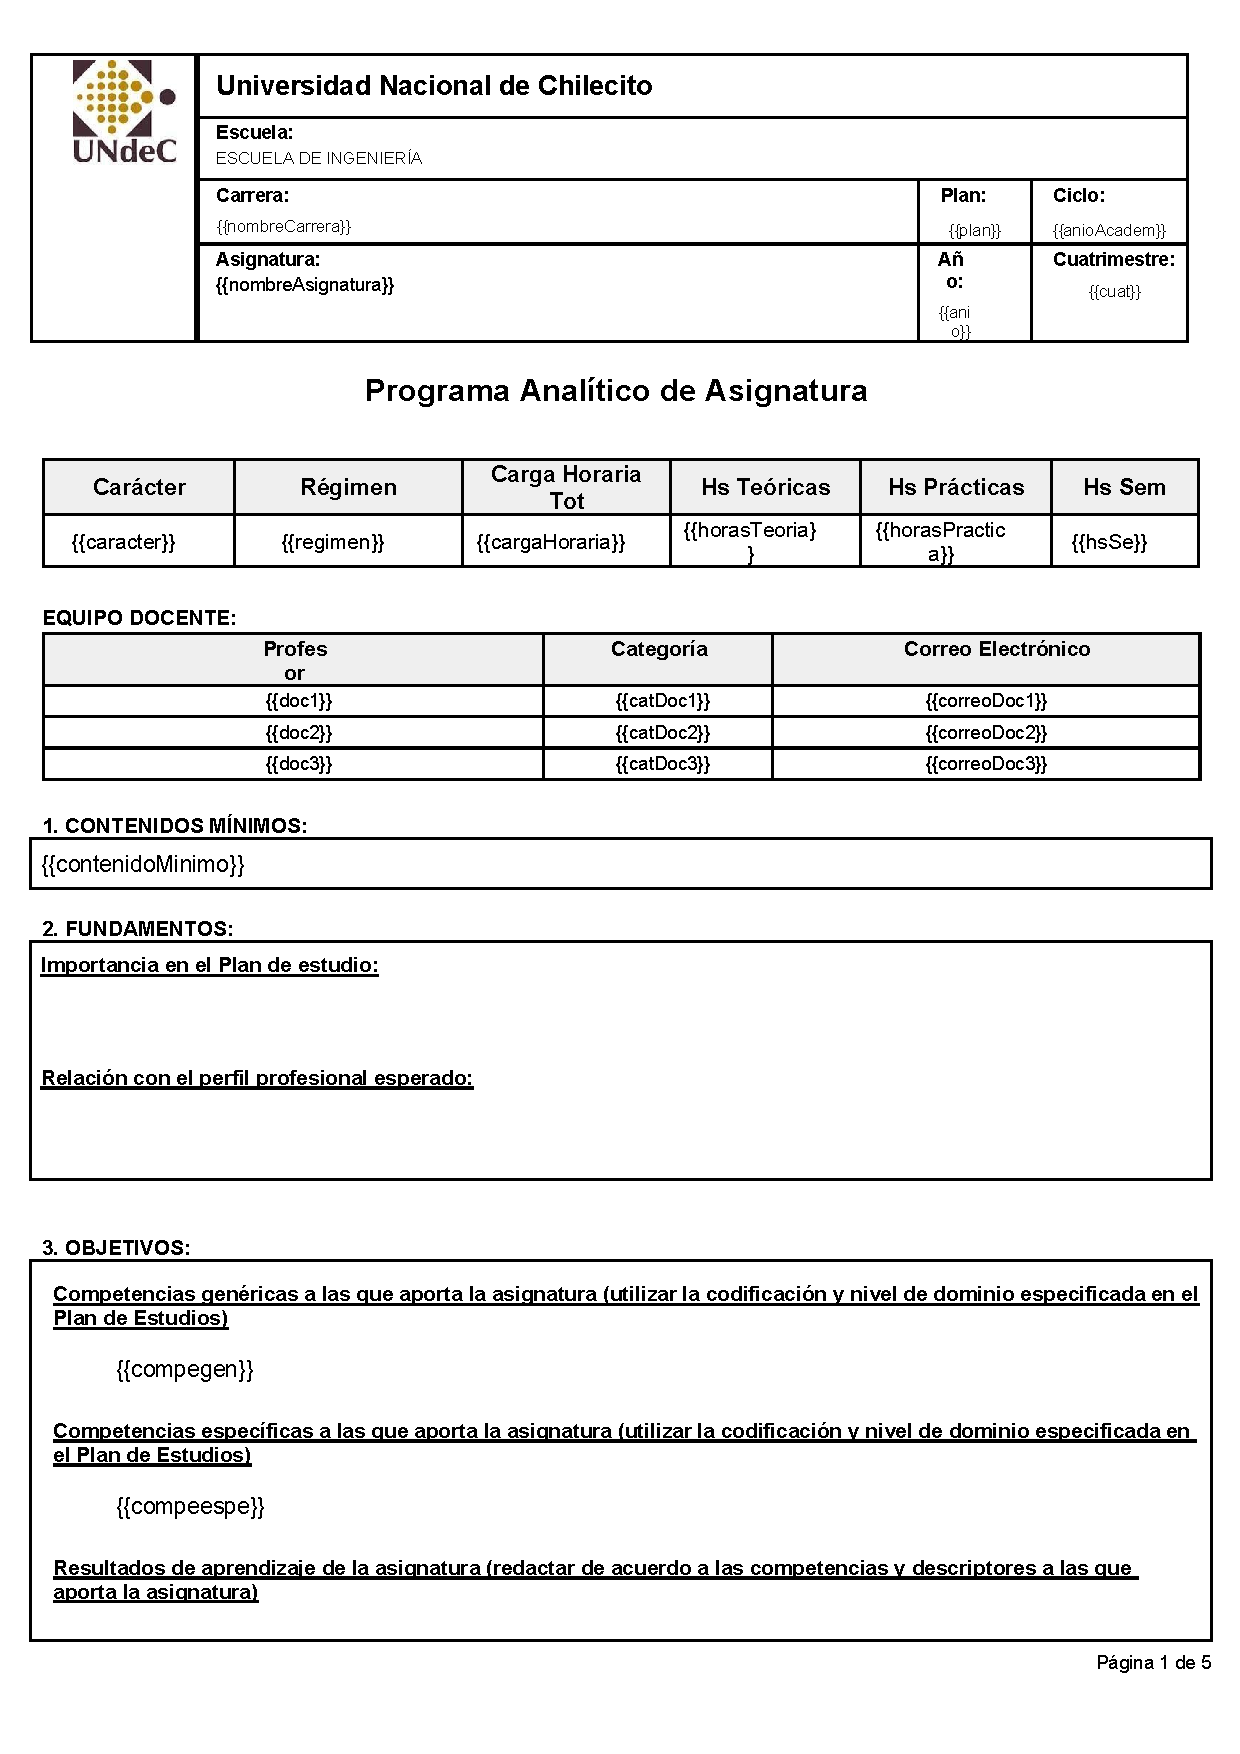
\includepdf[
  pages=-,
  pagecommand={},
  scale=0.82,
  frame=true,
  offset=0 0
]{figures/Template Propuestas.pdf}

%%─────────────────────────────────────────────────────────────────────────────
\chapter{Ejemplos de mensajes MCP (JSON-RPC)}
\label{anexo:mcp_ejemplos}
%%─────────────────────────────────────────────────────────────────────────────

% TODO: Mostrar ejemplos reales o representativos de mensajes MCP:
%
%   Ejemplo 1: Solicitud de tool
%     { "jsonrpc": "2.0", "method": "tools/call", "params": {...}, "id": 1 }
%
%   Ejemplo 2: Respuesta exitosa de tool
%     { "jsonrpc": "2.0", "result": {...}, "id": 1 }
%
%   Ejemplo 3: Invocación de resource
%     { "jsonrpc": "2.0", "method": "resources/read", "params": {...}, "id": 2 }
%
%   Ejemplo 4: Error en mensaje RPC
%     { "jsonrpc": "2.0", "error": {"code": -32601, "message": "Method not found"}, "id": 3 }

\section*{Mensaje de invocación de tool}

Este es un ejemplo de cómo el \textit{Host} invoca un tool a través del MCP Client:

\begin{lstlisting}
{
  "jsonrpc": "2.0",
  "method": "tools/call",
  "params": {
    "name": "extract_proposal",
    "arguments": {"docx_path": "/uploads/proposal.docx"}
  },
  "id": 1
}
\end{lstlisting}

% SECTION: Respuesta de tool
% TODO: Completar con ejemplos reales de respuestas

% SECTION: Manejo de errores
% TODO: Mostrar códigos de error JSON-RPC -32600 a -32603

%%─────────────────────────────────────────────
\chapter{Corpus de evaluación}
\label{anexo:corpus}
%%─────────────────────────────────────────────

% TODO: Describir el corpus en detalle (sin incluir los documentos completos
%   por razones de privacidad institucional):
%   - Tabla con características de las N propuestas evaluadas:
%     Propuesta | Año lectivo | Nº páginas | Nº campos presentes |
%     Formato (DOCX v1/v2/v3) | Observaciones
%   - Distribución de campos presentes/ausentes en el corpus
%   - Ejemplos ANONIMIZADOS de secciones problemáticas para el extractor
%   - Criterios de anotación del ground truth
\ldots

%%─────────────────────────────────────────────
\chapter{Instrucciones de instalación y puesta en marcha}
\label{anexo:instalacion}
%%─────────────────────────────────────────────

% TODO: Guía técnica de instalación para un nuevo entorno:
%   REQUISITOS:
%   - Python 3.11+, Node.js 20+, Git
%   - Clave de API de OpenAI
%
%   BACKEND:
%   cd backend
%   python -m venv .venv
%   .venv\Scripts\activate
%   pip install -r requirements.txt
%   cp .env.example .env   # completar OPENAI_API_KEY
%   python init_db.py
%   uvicorn app.main:app --reload --host 127.0.0.1 --port 8011
%
%   FRONTEND:
%   cd frontend
%   npm install
%   npm run dev -- --host 127.0.0.1 --port 5173
%
%   VERIFICACIÓN:
%   - Backend: http://127.0.0.1:8011/docs (Swagger UI)
%   - Frontend: http://127.0.0.1:5173
%
%   Usar \begin{lstlisting}[language=bash] para los bloques de comando
\ldots
